\section{Initial volume}
 \begin{figure}[H]
  \centering
  \captionsetup{width=.8\linewidth} 
  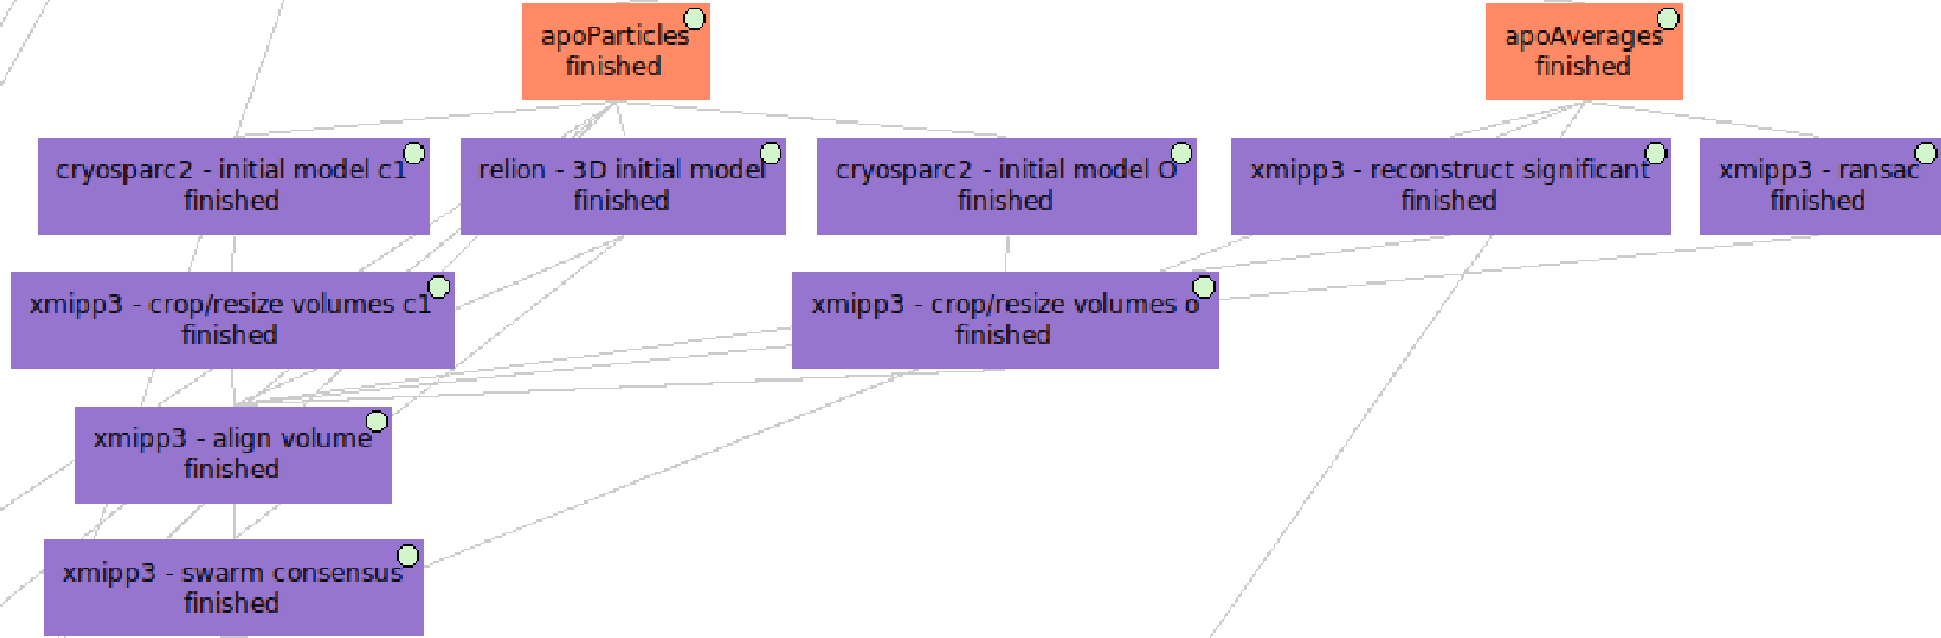
\includegraphics[width=1\textwidth]
  {{images/workflow_5.pdf}}
  \caption{Initial volume (Purple color).}
  \label{fig:workflow_5}
  \end{figure}

Right angles of each projection image are needed in order to reconstruct the \ttt{3D} map. In \ttt{3DEM}, however, these angles are unknown and we have to estimate them. The most popular way of estimating them is comparing the projections of a  volume similar to ours, known as initial volume, with the images obtained from the microscope. Since the 3D map reconstruction process requires an approximate low resolution map to be refined in further steps according to the projection images of particles, in this tutorial we are going to generate a $de-novo$ initial map model combining the results obtained by different algorithms: First, to compute the initial volume using the set of aligned particles as input, we have used $cryoSPARC$ \ttt{Stochastic Gradient Descent (SGD)} and $Relion$ \ttt{Stochastic Gradient Descent (SGD)} (\ffigure{fig:workflow_5}, left). Second, to generate the initial volume from the class representative particles, we have run $Xmipp$ \ttt{reconstruct significant} and $Xmipp$ \ttt{RANSAC} (\ffigure{fig:workflow_5}, right). $Xmipp$ \ttt{reconstruct significant} sets the map in a \ttt{Weighted Least Square} framework and calculates weights through a statistical approach based on the cumulative density function of different image similarity measures. $Xmipp$ \ttt{RANSAC} is based on an initial non-lineal dimension reduction approach with which selecting sets of class representative images that capture the most of the structural information of each particle. These reduced sets will be used to build maps starting from random orientation assignments. The best map will be selected from these previous assumptions using a random sample consensus (RANSAC) approach.\\

\subsection*{$cryoSPARC$ \ttt{Stochastic Gradient Descent (SGD)}}
The algorithm $cryoSPARC$ \ttt{Stochastic Gradient Descent (SGD)} has been implemented in the protocol \scommand{cryosparc2-initial model}, that we execute twice with two different values for params \ttt{Number of Ab-Initio classes} and \ttt{Symmetry} (\ttt{Ab-initio reconstruction} tap of \ffigure{fig:initial_vol_1} and \ffigure{fig:initial_vol_3}). The set of particles selected in the previous step is used as input in both cases (see the \ttt{Input} tap of the protocol form). 

\begin{figure}[H]
  \centering
  \captionsetup{width=.8\linewidth} 
  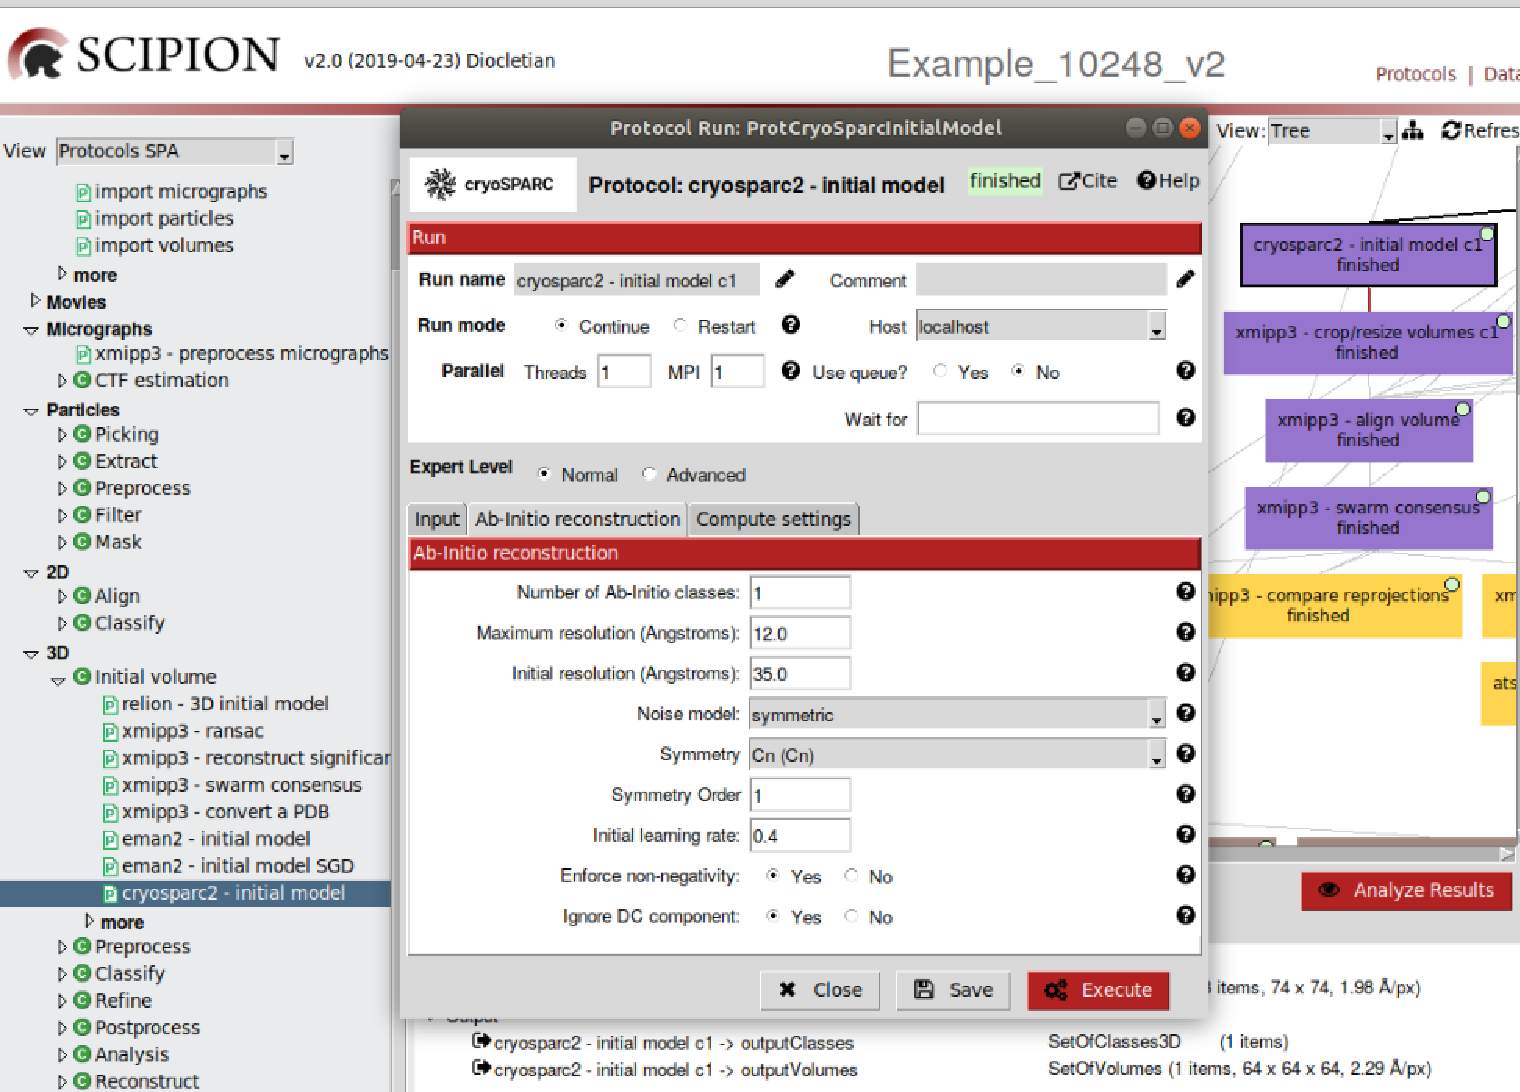
\includegraphics[width=0.95\textwidth]
  {images/initial_vol_1.pdf}
  \caption{Completing the second tap of the protocol \scommand{cryosparc2-initial model} with one \ttt{Ab-Initio} class and no \ttt{Symmetry}.}
  \label{fig:initial_vol_1}
  \end{figure}
  
In the first case, only one \ttt{Ab-Initio} class has been selected and \ttt{C1 Symmetry} has been considered (\ffigure{fig:initial_vol_1}). In the second one, instead, three \ttt{Ab-Initio classes} and octaheadral \ttt{Symmetry} have been selected (\ffigure{fig:initial_vol_3}). Each \ttt{Ab-Initio} class will be randomly initialized, unless an initial map is provided. In that case, each class will be a random variant of the initial map. Regarding symmetries, enforcing symmetry above C1 is not recommendable for $ab-initio$ reconstructions.

\begin{figure}[H]
  \centering
  \captionsetup{width=.8\linewidth} 
  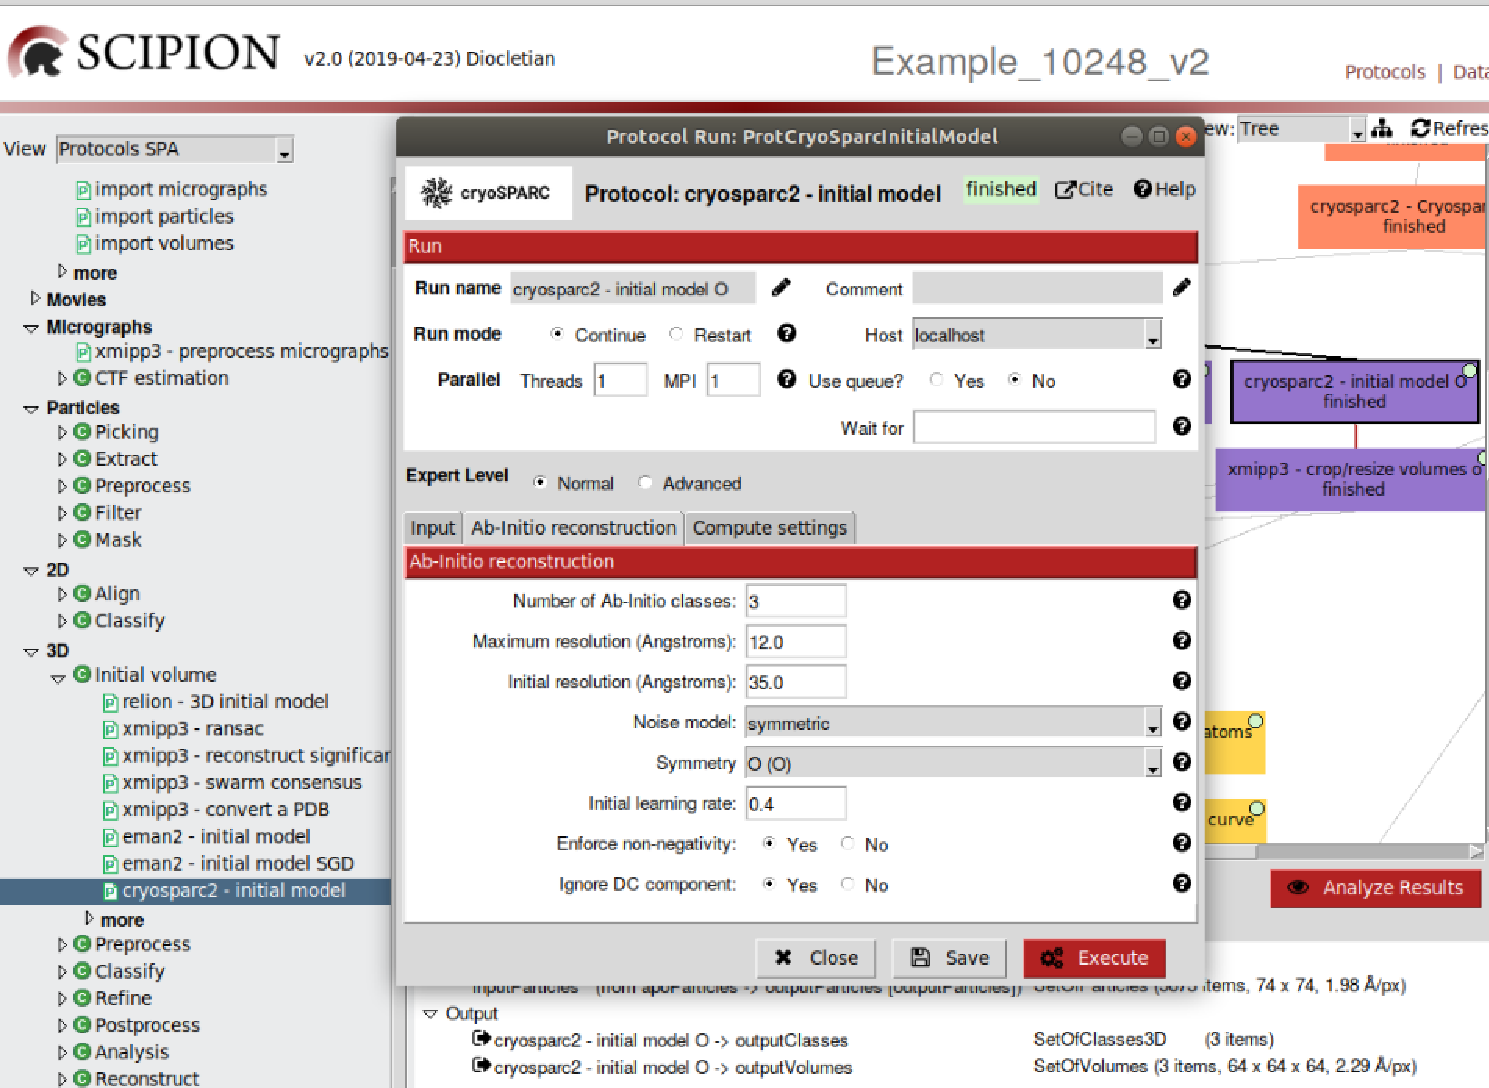
\includegraphics[width=0.95\textwidth]
  {images/initial_vol_3.pdf}
  \caption{Filling in the second tap of the protocol \scommand{cryosparc2-initial model} with three \ttt{Ab-Initio classes} and octahedral \ttt{Symmetry}.}
  \label{fig:initial_vol_3}
  \end{figure}
  
Maps or \ttt{3D} classes generated can be appreciated by pressing \scommand{Analyze Results}. One map has been generated in the first case and three in the second one, although only one of these three maps has been built with most of particles (5,643).\\

Since the size and sampling rate of maps generated with \scommand{cryosparc2-initial model} differ from the size and sampling rate of the input particles, a resizing intermediate method has to be applied to recover these dimensions. Protocol \scommand{xmipp3-crop/resize volumes} will hep us with this task (\ffigure{fig:crop_resize}). As input, select the output volume\/s of the previous protocols, \ttt{Dimensions} for \ttt{Resize option}, and 74 pixels as \ttt{New image size}.

\begin{figure}[H]
  \centering
  \captionsetup{width=.8\linewidth} 
  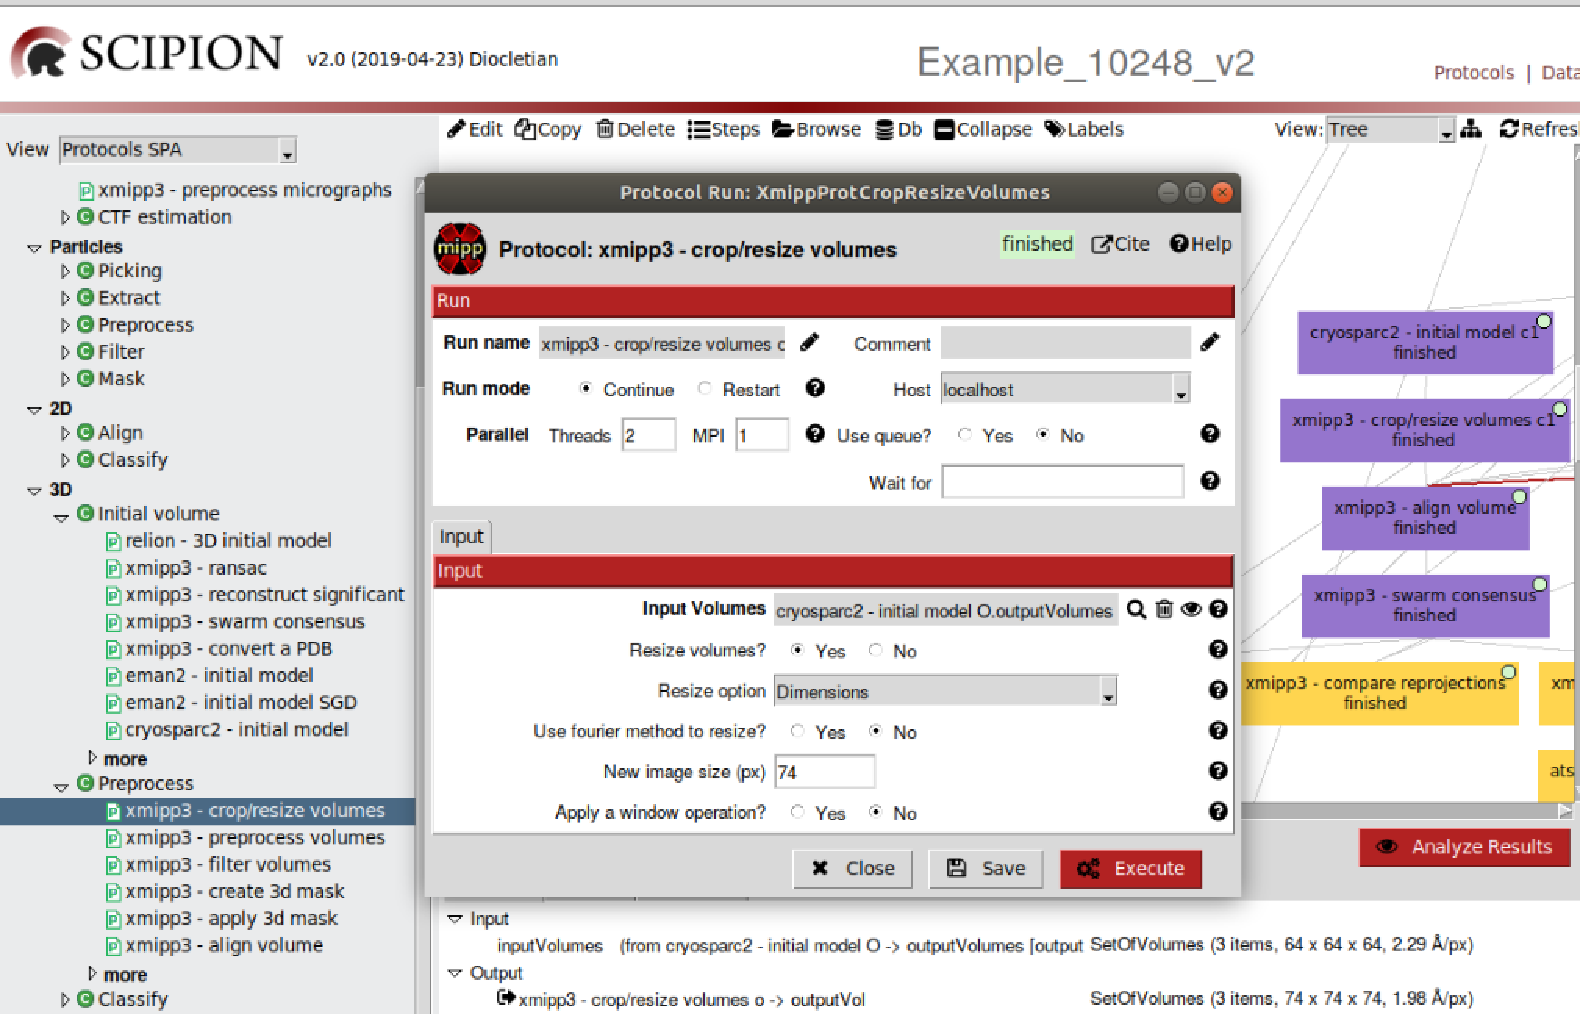
\includegraphics[width=0.95\textwidth]
  {images/crop_resize.pdf}
  \caption{Completing the protocol \scommand{xmipp3-crop/resize volumes}.}
  \label{fig:crop_resize}
  \end{figure}

\subsection*{$Relion$ \ttt{Stochastic Gradient Descent (SGD)}}
$Relion$ \ttt{Stochastic Gradient Descent (SGD)} has been implemented in the protocol \scommand{relion-3D initial model}. Fill in the param values and execute it (\ffigure{fig:initial_vol_2}). 

\begin{figure}[H]
  \centering
  \captionsetup{width=.8\linewidth} 
  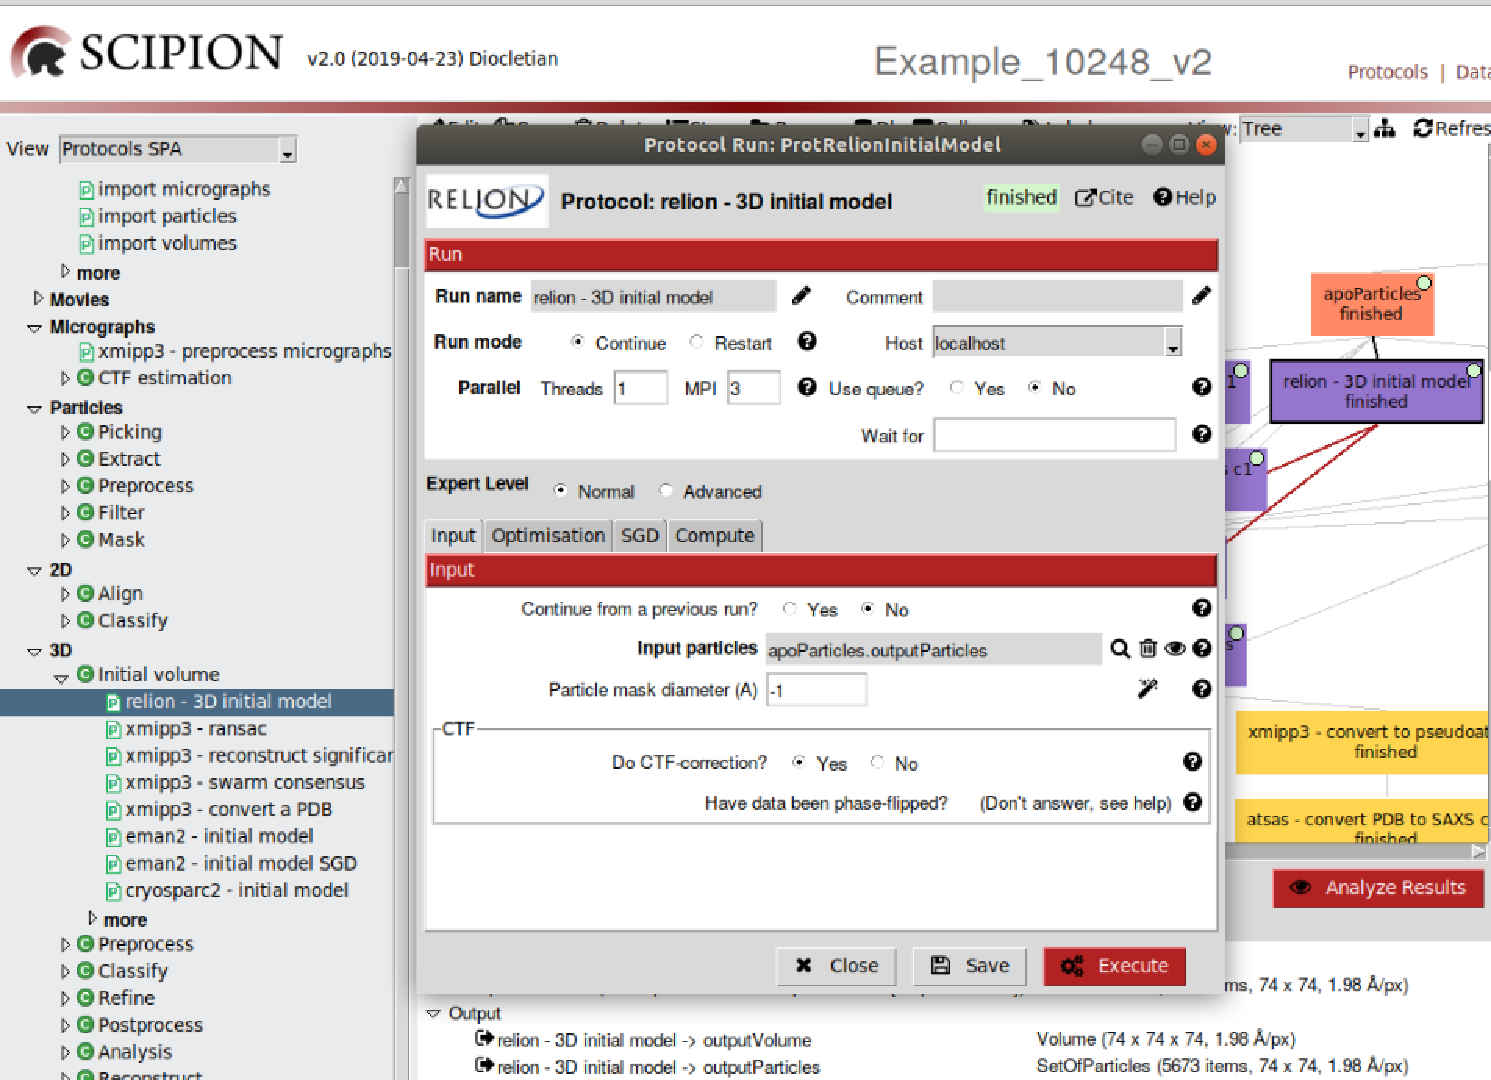
\includegraphics[width=0.95\textwidth]
  {images/initial_vol_2.pdf}
  \caption{Filling in the \ttt{Input} tap of the protocol \scommand{relion-3D initial model}.}
  \label{fig:initial_vol_2}
  \end{figure}

  Only one volume has been generated with this protocol that keeps size and sampling rate of the input particles. You can visualize it with \chimera in 3D by pressing \scommand{Analyze Results} and selecting in the \ttt{Volumes} box \ttt{Display volume with} \ttt{chimera}. 
  
\subsection*{$Xmipp$}
Using the 14 class representative particles as input, as well as the type of symmetry (octahedral), the protocol \scommand{xmipp3-reconstruct significant} (\ffigure{fig:xmipp_reconstruct_significant}) also generates one initial volume and preserves the size and samplig rate of the input \ttt{2D} classes.

\begin{figure}[H]
  \centering
  \captionsetup{width=.8\linewidth} 
  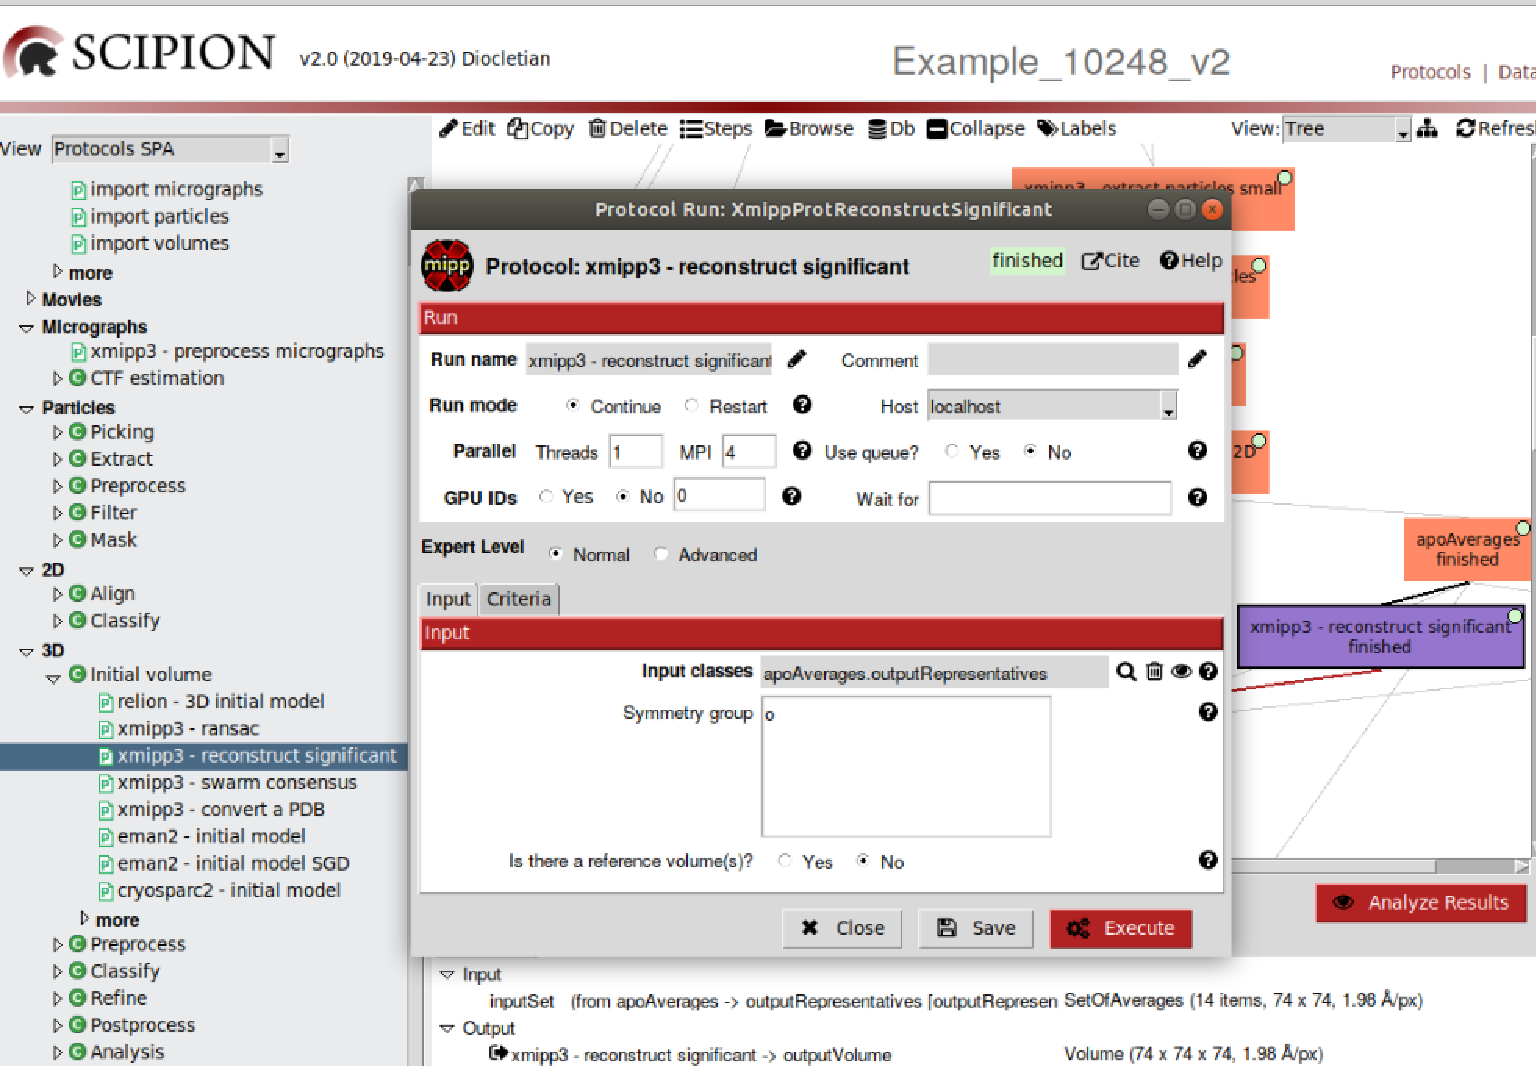
\includegraphics[width=0.95\textwidth]
  {images/xmipp_reconstruct_significant.pdf}
  \caption{Completing the \ttt{Input} tap of the protocol \scommand{xmipp3-reconstruct significant}.}
  \label{fig:xmipp_reconstruct_significant}
  \end{figure}

$Xmipp$ \ttt{RANSAC} algorithm, implemented in the protocol \scommand{xmipp3-ransac} (\ffigure{fig:xmipp_ransac}), although starts from the same input than $Xmipp$ \ttt{reconstruct significant}, generates 10 different maps and preserves the size and sampling rate from the input \ttt{2D} classes. You can choose a different number of output maps in the advanced param \ttt{Number of best volumes to refine}.

\begin{figure}[H]
  \centering
  \captionsetup{width=.8\linewidth} 
  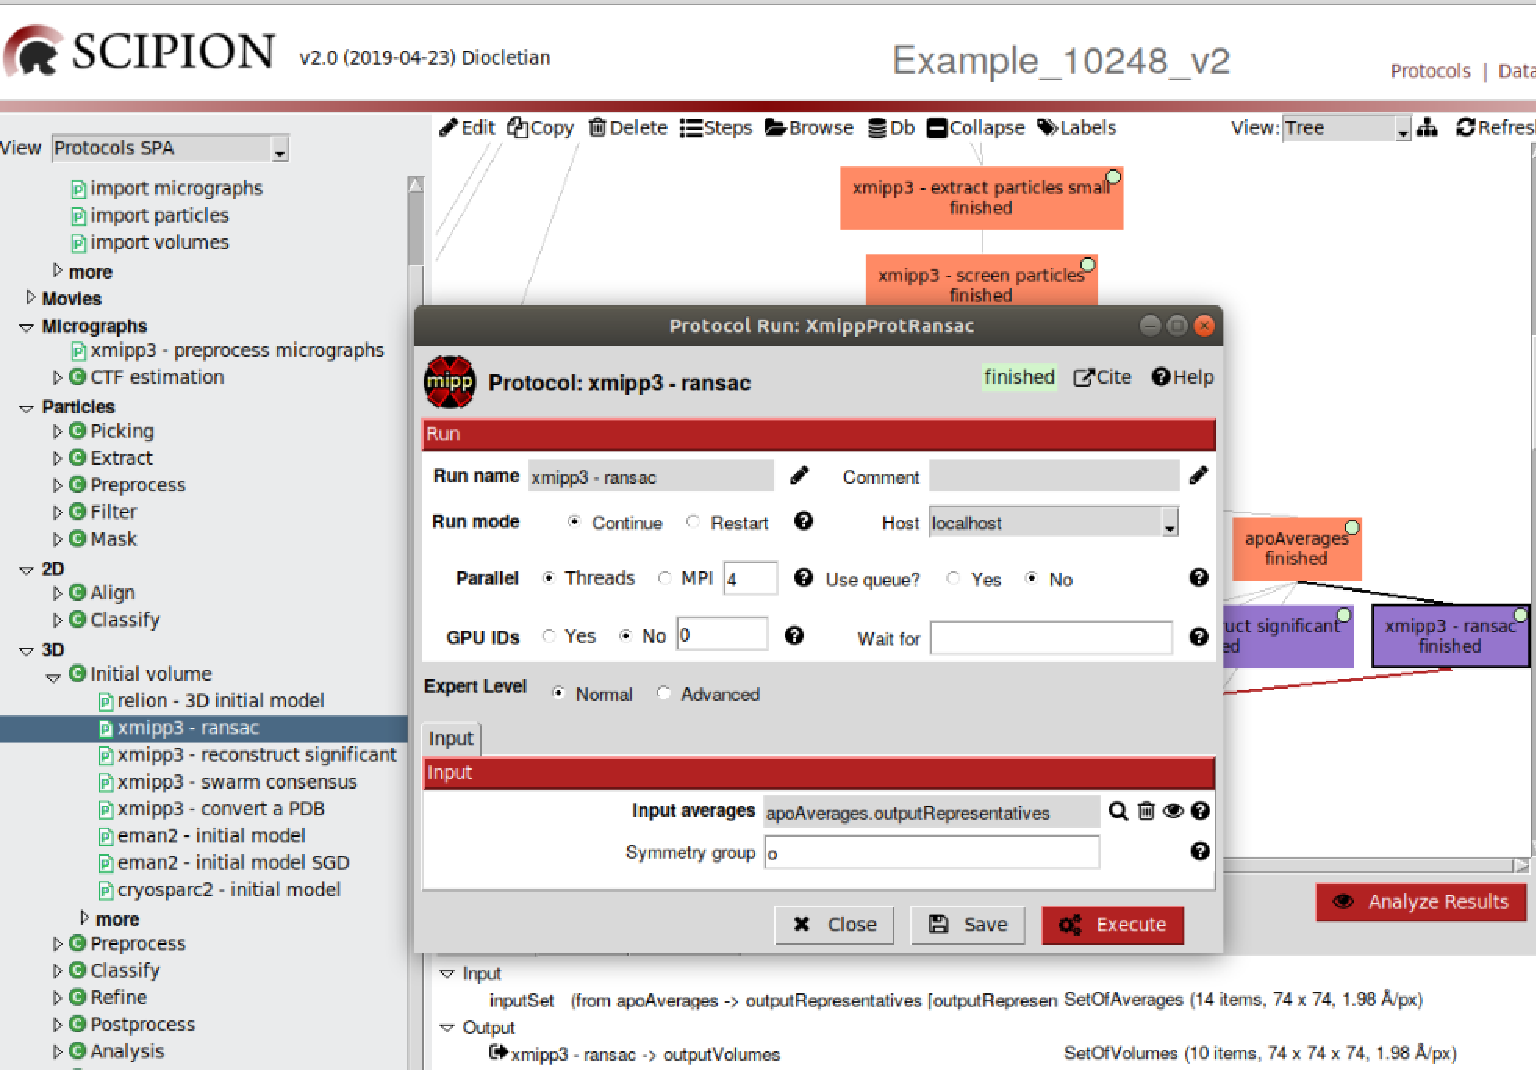
\includegraphics[width=0.95\textwidth]
  {images/xmipp_ransac.pdf}
  \caption{Filling in the params of the protocol \scommand{xmipp3-ransac}.}
  \label{fig:xmipp_ransac}
  \end{figure}
  
\subsection*{Map alignment and swarm consensus}
Next, we perform a local alignment of the 16 maps generated, starting both from particles and \ttt{2D} classes, using the protocol \scommand{xmipp3-align volume} (\ffigure{fig:align_volume}). As \ttt{Reference volume} we select the initial volume obtained by the $Relion$ algorithm.

\begin{figure}[H]
  \centering
  \captionsetup{width=.8\linewidth} 
  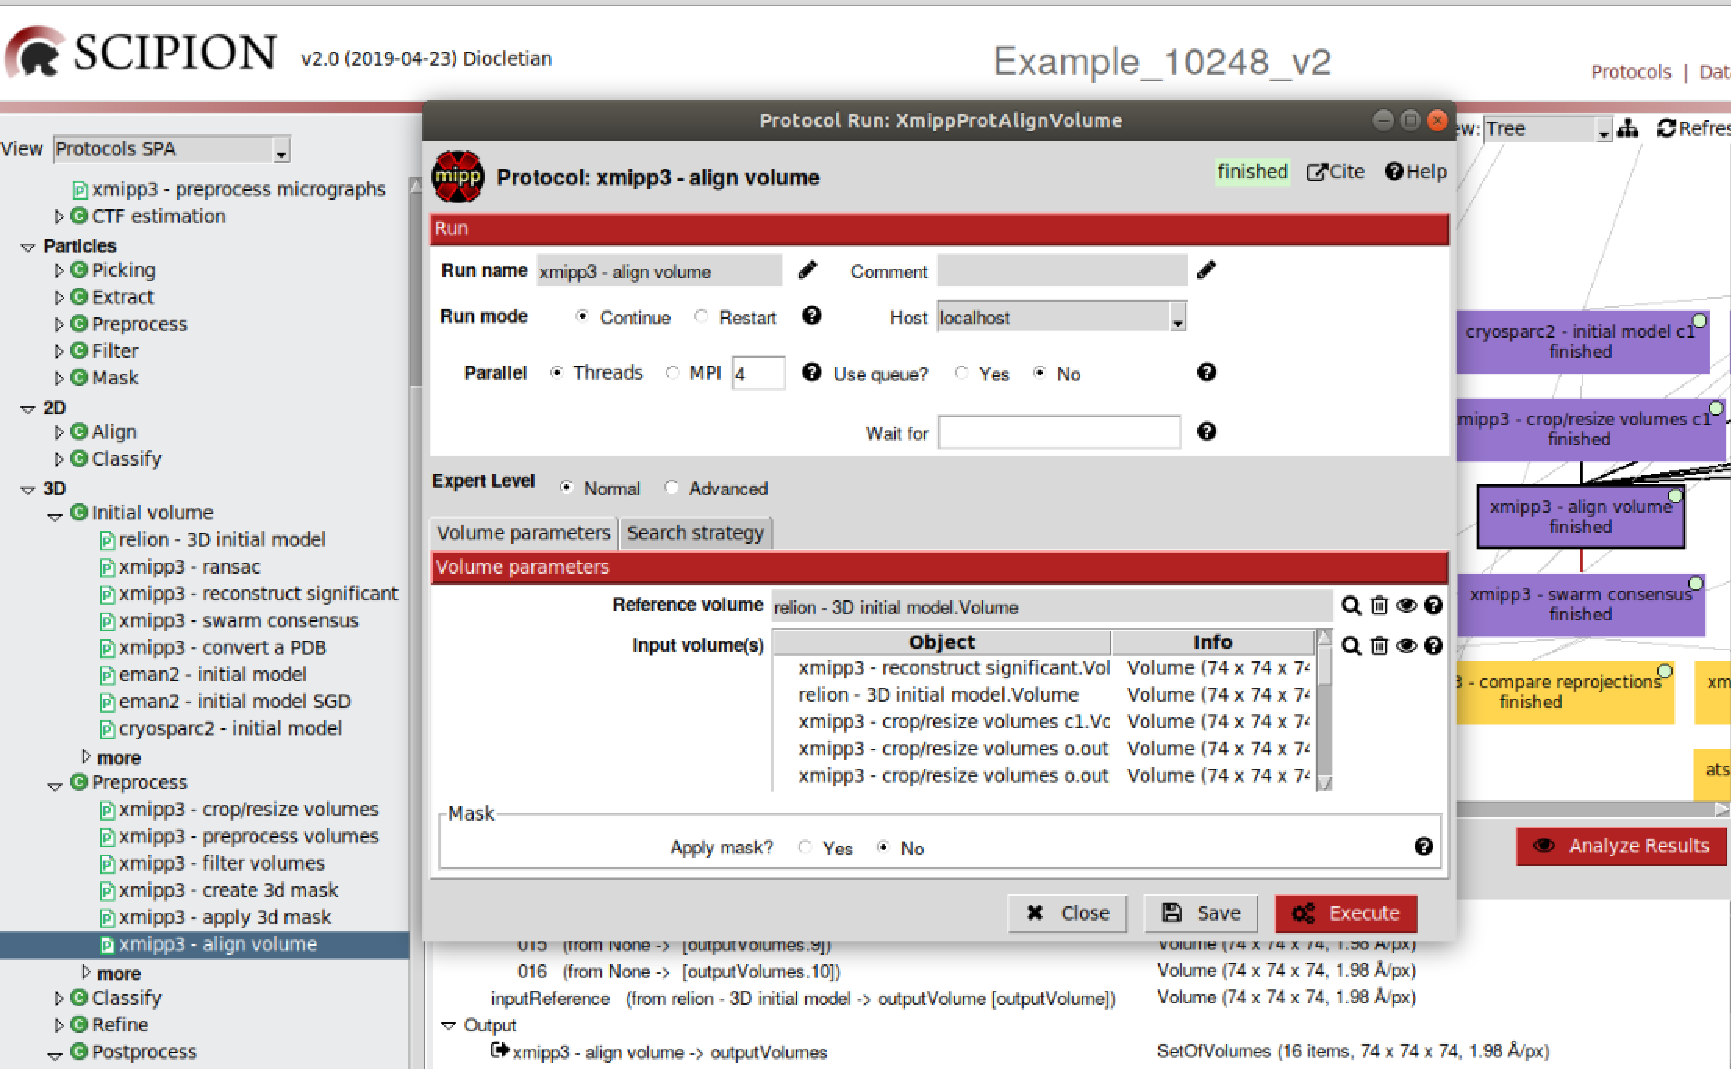
\includegraphics[width=0.95\textwidth]
  {images/align_volume.pdf}
  \caption{Completing the params of the protocol \scommand{xmipp3-align volume}.}
  \label{fig:align_volume}
  \end{figure}
  
A new set of 16 maps has been created keeping the same size and sampling rate shown by the initial particles. These maps can be visualized by pressing \scommand{Analyze Results}.\\

Next, in order to have only one initial volume partially refined against the selected set of particles, we use the protocol \scommand{xmipp3-swarm consensus} (\ffigure{fig:swarn_consensus}). The inputs of this is a 3D refinement protocol are the set of 16 maps and the set of 5,673 $Relion$ extracted particles, previously generated. In this case maps and particles have the same size and sampling rate. The program try to optimize the correlation between the swarm of volumes and the set of particles. Only a fraction of the particles are used to update this stochastic maximization.

\begin{figure}[H]
  \centering
  \captionsetup{width=.8\linewidth} 
  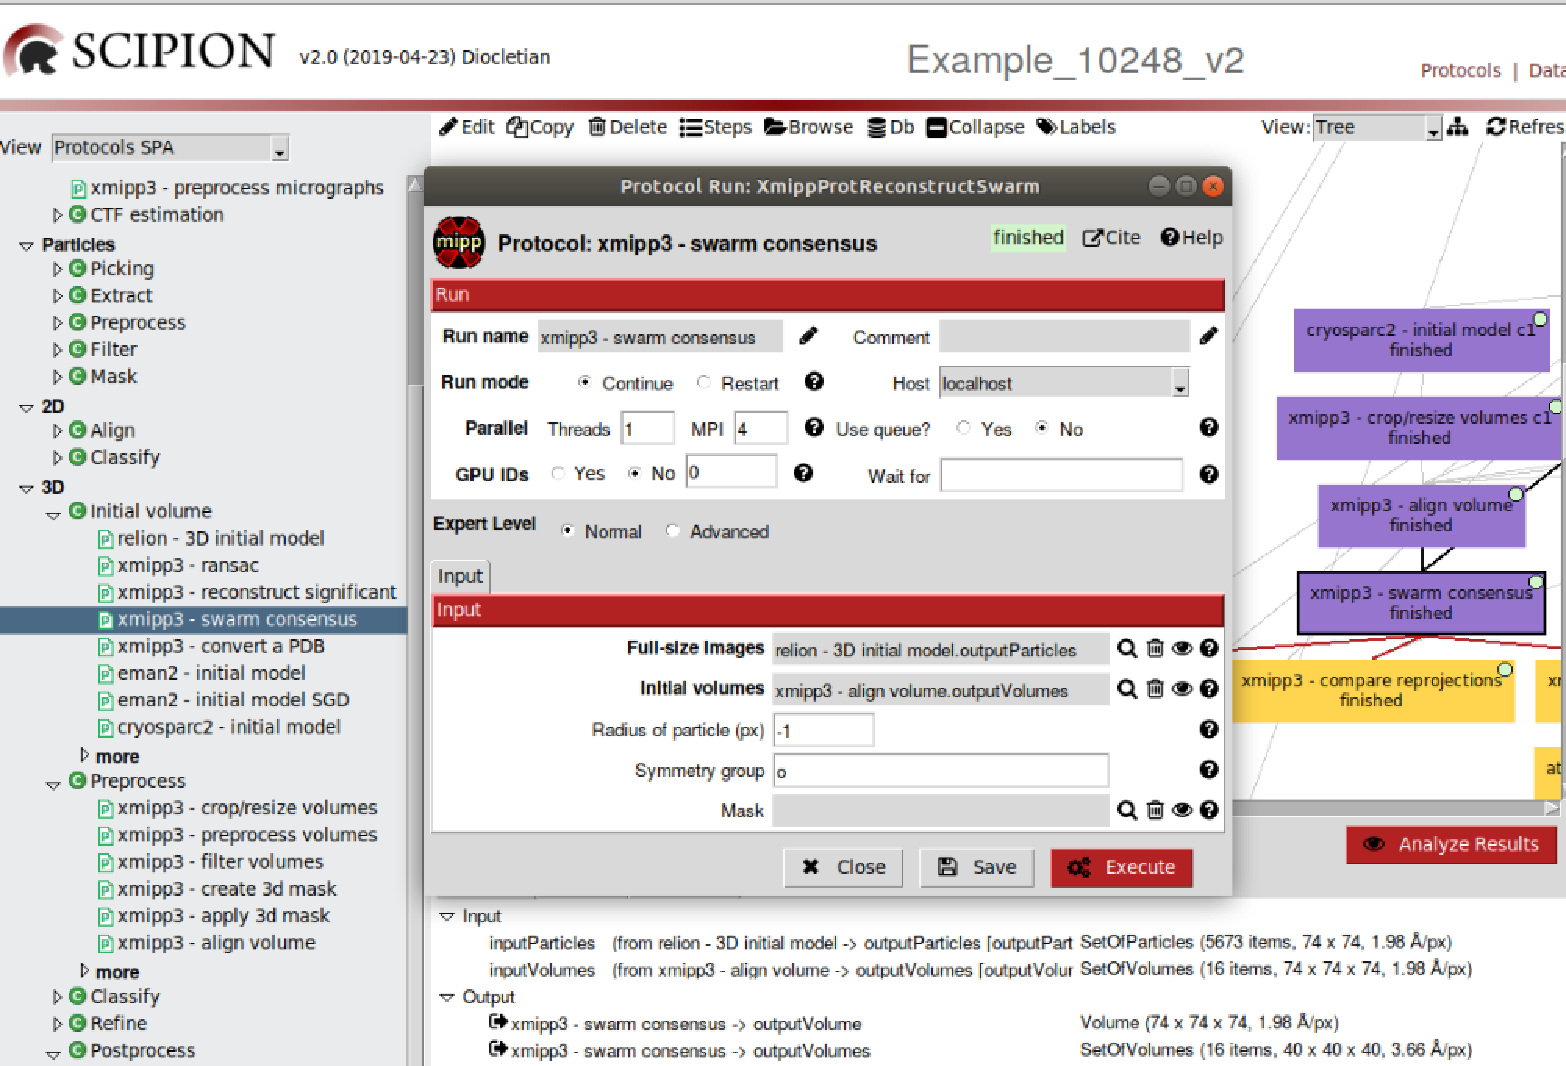
\includegraphics[width=0.95\textwidth]
  {images/swarn_consensus.pdf}
  \caption{Filling in the params of the protocol \scommand{xmipp3-swarm consensus}.}
  \label{fig:swarn_consensus}
  \end{figure}
  
After 15 iterations, this protocol generates two outputs, 16 downsampled maps and a map with the size and sampling rate of the inputs. This map will be the initial volume that will be further refined.\\

\subsection*{Validation of the initial volume}
To check the reliability of this initial volume, we can compare its projection images with the set of representative \ttt{2D} classes using the protocol \scommand{xmipp3-compare reprojections} (\ffigure{fig:xmipp_compare_reprojections}). \ttt{Symmetry group} has to be also included in the input form. This \ttt{3D} validation protocol computes residues, $i.e.$, differences between the experimental images and reprojections, as well as other statistics. The values of these statistics might suggest the presence of outliers.

\begin{figure}[H]
  \centering
  \captionsetup{width=.8\linewidth} 
  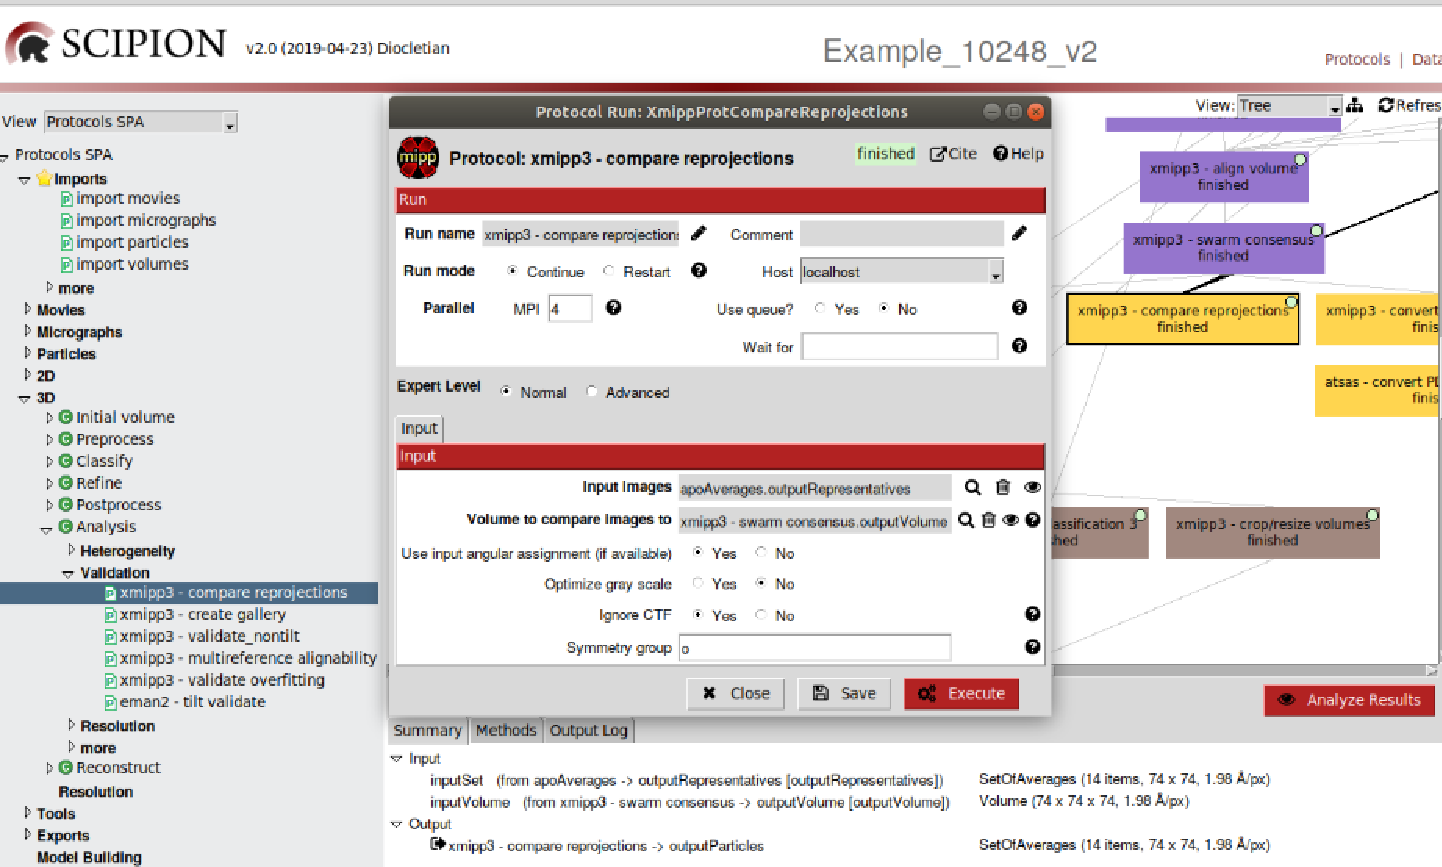
\includegraphics[width=0.95\textwidth]
  {images/xmipp_compare_reprojections.pdf}
  \caption{Completing the params of the protocol \scommand{xmipp3-compare reprojections}.}
  \label{fig:xmipp_compare_reprojections}
  \end{figure}
  
In our example, values of \ttt{\_xmipp\_cost} between 0.8115 and 0.8725 (press \scommand{Analyze Results}) suggest quite good similarity among initial volume projection images and the set of 14 \ttt{2D} classes.\\

\subsection*{From the initial volume to a pseudoatom structure}
The initial map can also be used to generate an initial pseudoatom structure that can be used to infer the SAXS (Small-Angle X-ray Scattering). Two consecutive executed protocols perform these two tasks, \scommand{xmipp3-convert to pseudoatoms} and \scommand{xmipp3-convert to pseudoatoms}.\\

The protocol \scommand{xmipp3-convert to pseudoatoms} (\ffigure{fig:xmipp_convert_to_pseudoatoms}) requires the initial map, previously computed, and the \ttt{Pseudoatom radius (vox)} as inputs.

\begin{figure}[H]
  \centering
  \captionsetup{width=.8\linewidth} 
  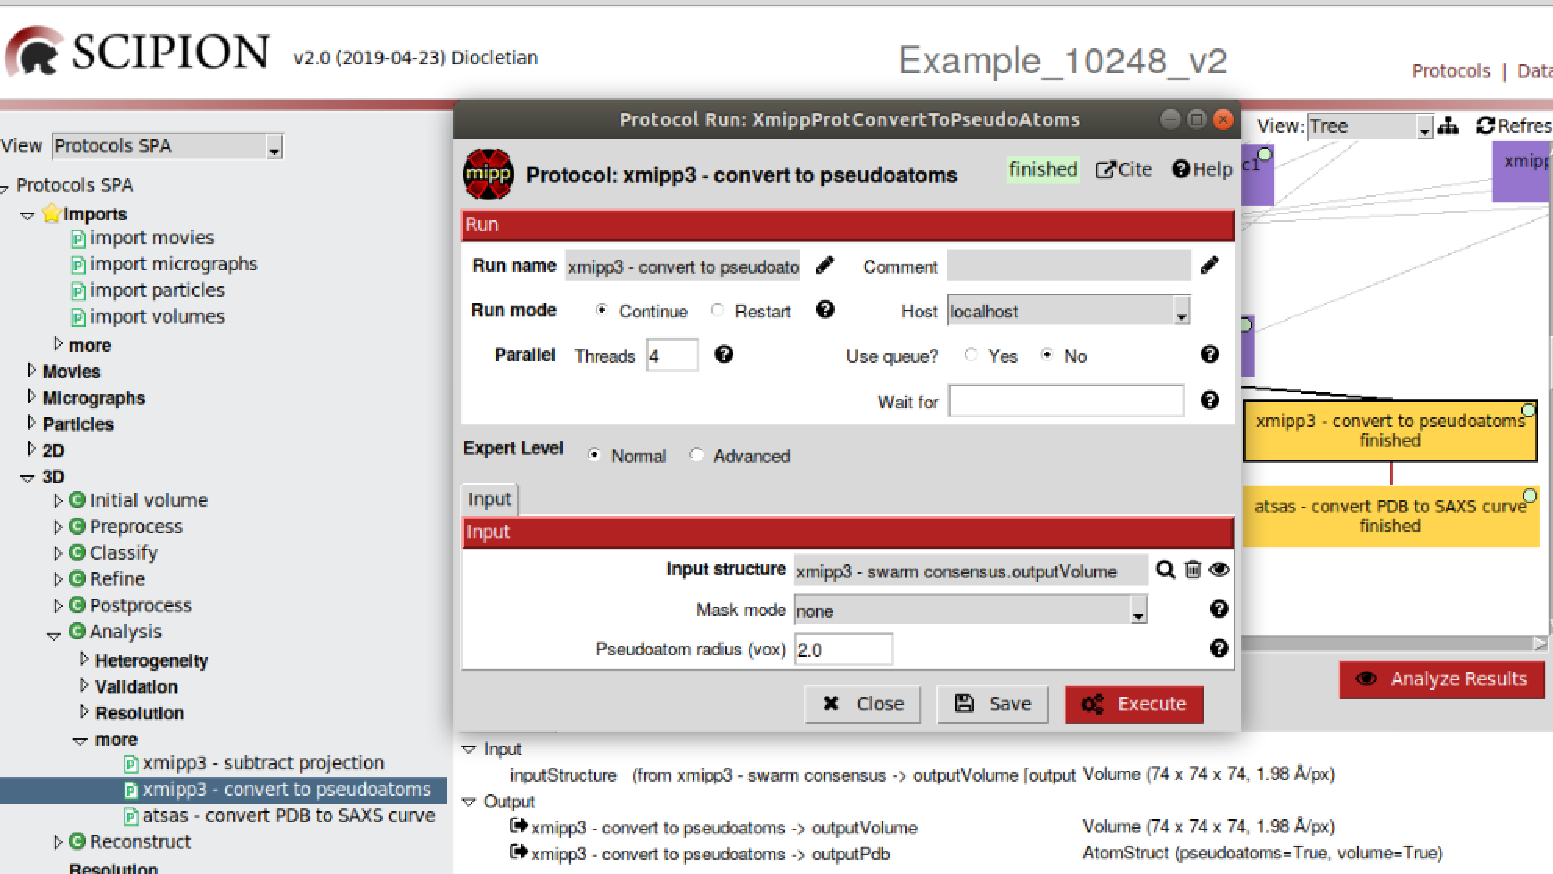
\includegraphics[width=0.95\textwidth]
  {images/xmipp_convert_to_pseudoatoms.pdf}
  \caption{Filling in the params of the protocol \scommand{xmipp3-convert to pseudoatoms}.}
  \label{fig:xmipp_convert_to_pseudoatoms}
  \end{figure}

The pseudoatomic structure obtained can be visualized with \chimera (press \scommand{Analyze Results}. This pseudoatom structure can be used as input of the protocol \scommand{atsas-convert PDB to SAXS} (\ffigure{fig:atsas_convert_PDB_to_SAXS}) to generate the respective SAXS curves by running the program $Crysol$ from $Atsas$ \citep{svergun1995crysol}. Press {Analyze results} to visualize the curves in solution and in vacuo.

\begin{figure}[H]
  \centering
  \captionsetup{width=.8\linewidth} 
  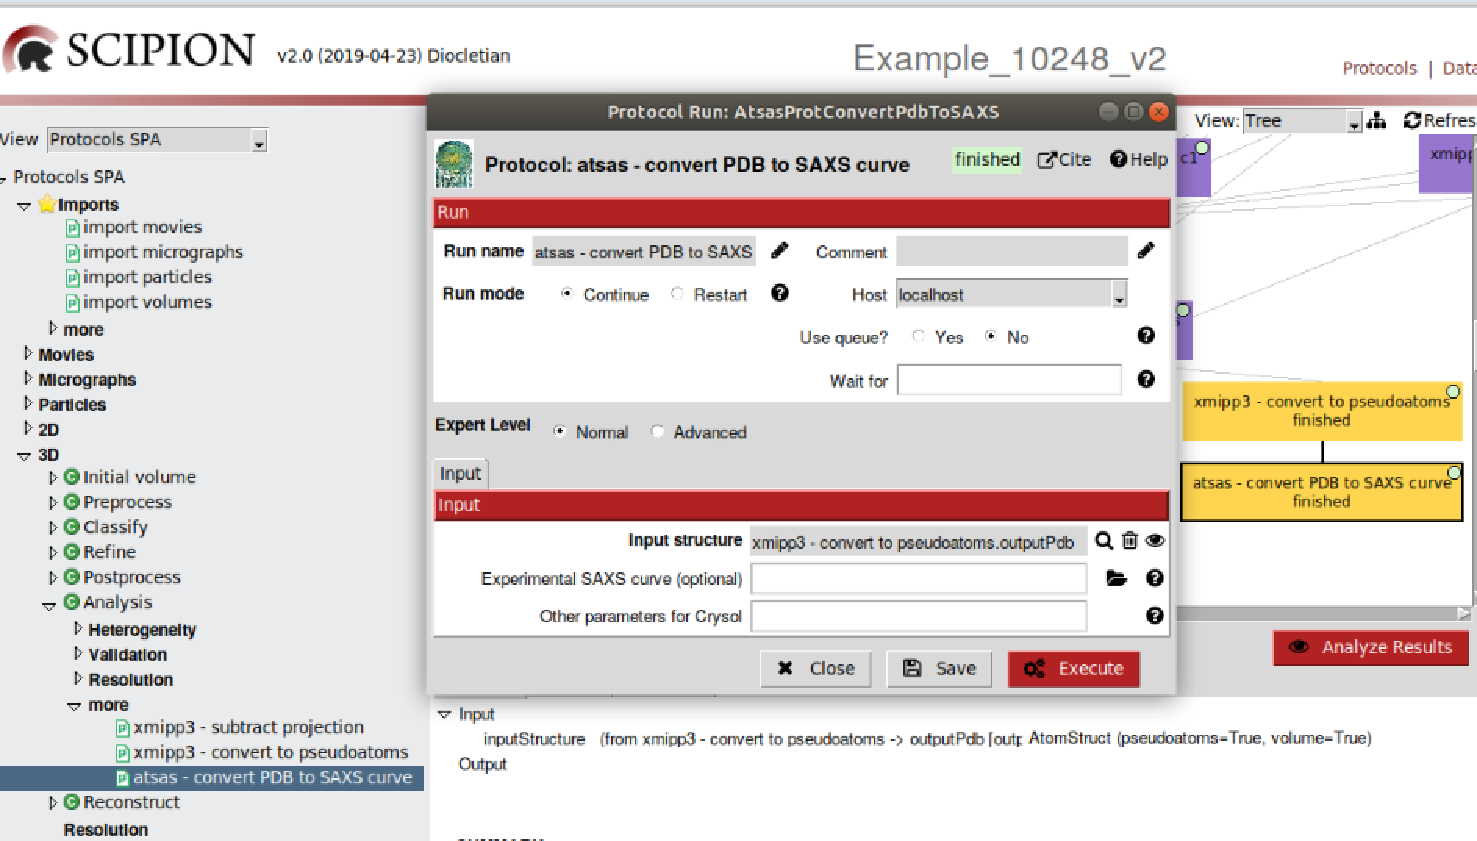
\includegraphics[width=0.95\textwidth]
  {images/atsas_convert_PDB_to_SAXS.pdf}
  \caption{Completing the params of the protocol \scommand{atsas-convert PDB to SAXS}.}
  \label{fig:atsas_convert_PDB_to_SAXS}
  \end{figure}


